\chapter{Коэффициент усиления}
\label{ch:chap2}

В соответствии с моим вариантом:
$$
    i=j=2, \tab W_1(s) = \frac{s-2}{s^2+6s+5}, \tab W_2(s) = \frac{-9s^3+16s^2-6s}{10s^3+12s^2+5s+1}
$$
Необходимо добавить к каждой функции коэффициент усиления $k > 0$.

\section{Передаточная функция $W_1$}
Для $k=1$:
$$
W_1(s) = \frac{1(s-2)}{s^2+6s+5},
$$
Рассчитаем полюса: $\lambda_{1,2} = \{-5, -1 \}$, значит разомкнутая система будет устойчива. 

Построим для неё годографы, с разными $k$:
\begin{figure}[ht]
    \centering
    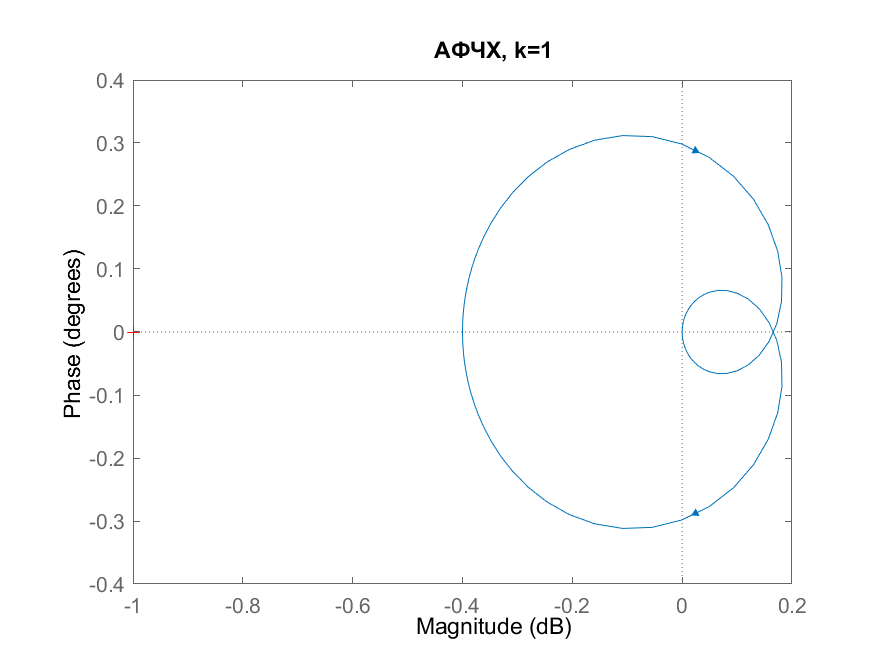
\includegraphics[width=0.7\textwidth]{nyquist_task21_object1.png}
    \caption{Годограф Найквиста для разомкнутой системы, $k=1$}
\end{figure}
\begin{figure}[ht]
    \centering
    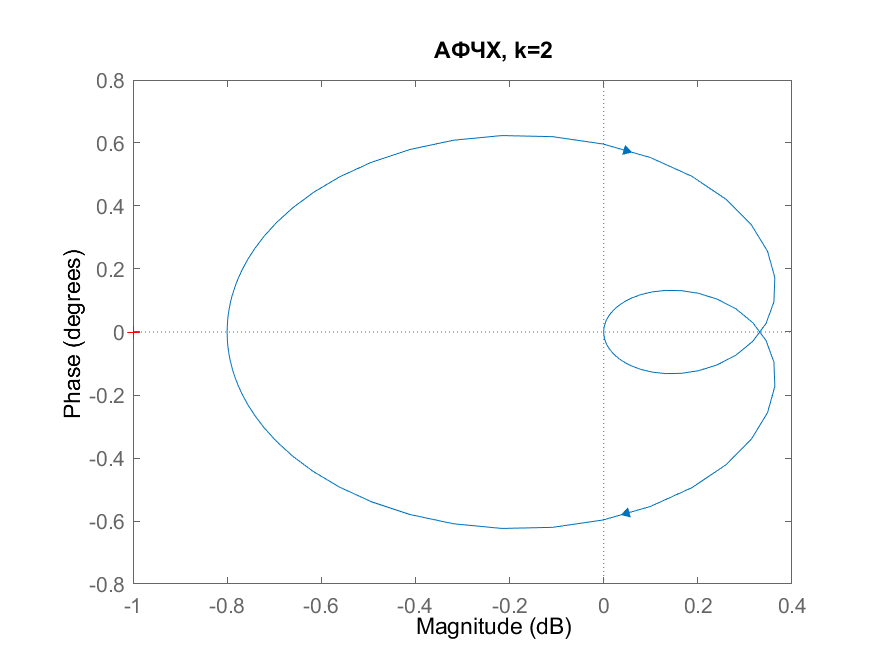
\includegraphics[width=0.7\textwidth]{nyquist_task22_object1.png}
    \caption{Годограф Найквиста для разомкнутой системы, $k=2$}
\end{figure}
\begin{figure}[ht]
    \centering
    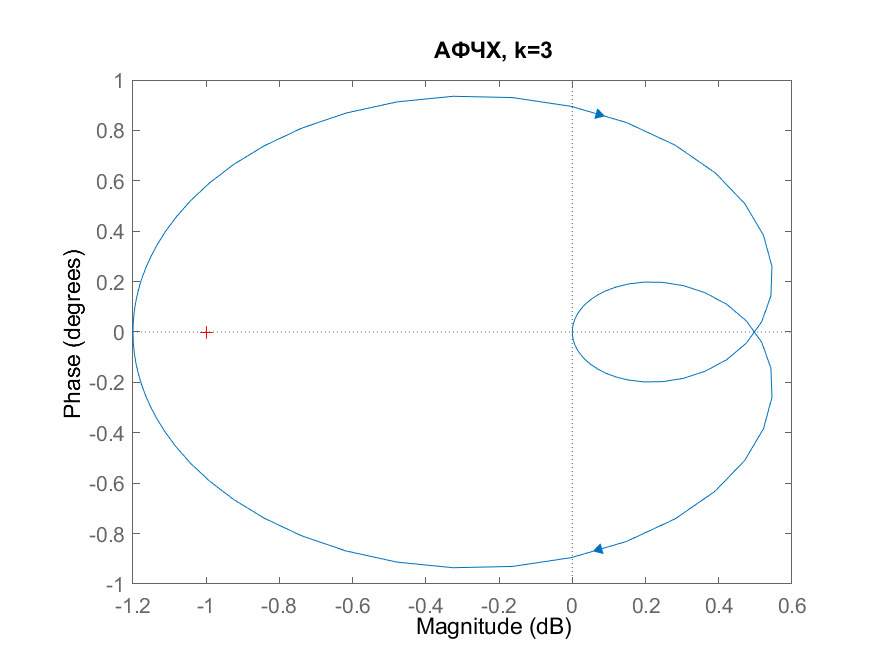
\includegraphics[width=0.7\textwidth]{nyquist_task23_object1.png}
    \caption{Годограф Найквиста для разомкнутой системы, $k=3$}
\end{figure}
\begin{figure}[ht]
    \centering
    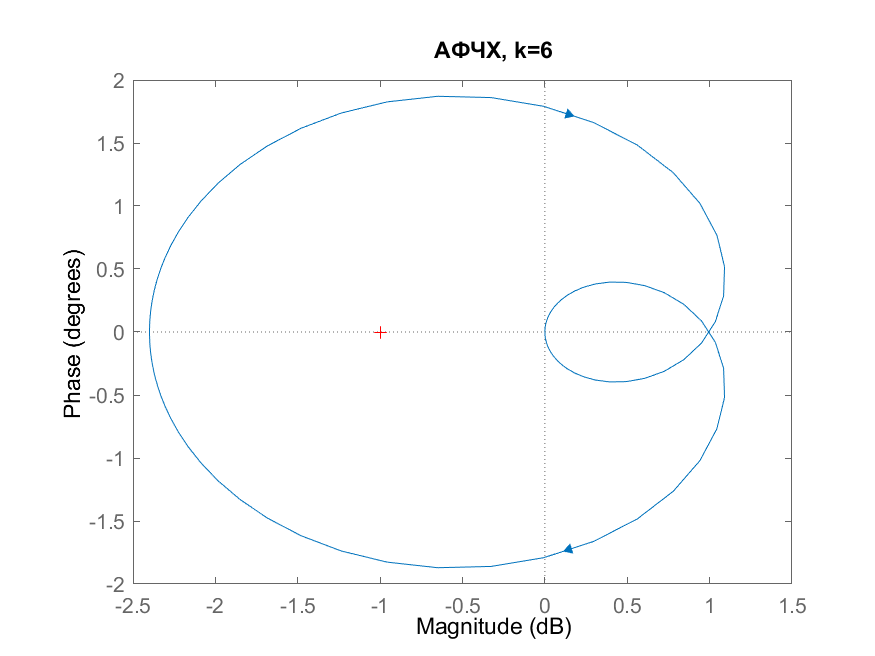
\includegraphics[width=0.7\textwidth]{nyquist_task24_object1.png}
    \caption{Годограф Найквиста для разомкнутой системы, $k=6$}
\end{figure}

Выходит, что коэффициент $k$ влияет на кривую годографа, расширяя её вдоль мнимой оси и влево по оси действительной части, в конце концов 
доходя критической точки $(-1,0)$.

Годограф делает обороты по часовой стрелки, а значит когда он дойдёт до критической точки, то замкнутая система приобретёт дополнительный несточивый полюс, когда коэффиент будет примерно $k > 2.5$ (критерий Найквиста).
Петля внутри не перемешается левее нуля при любом $k$, а значит мы максимум получим только один неустойчивый полюс, при $k > 2.5$.

Теперь проверим по критерию Гурвица это предположение:
$$
    W_{1,closed} = \frac{W_1}{1+W_1} = \frac{k(s-2)}{s^2 + (6+k)s + (5-2k)}
$$

$$
    \begin{cases}
        6+k > 0 \\
        5-2k > 0
    \end{cases} \to
    \begin{cases}
        k > -6 \\
        2.5 > k
    \end{cases}
$$
Но отрицательные значения мы не рассматриваем, поэтому по критерию Гурвица система будет асимптотически устойчива при $0 < k < 2.5$,
так как до этого значения годограф не захватывает точку $(-1, 0)$, а значит не добавляет дополнительный полюс.
\newpage
\subsection{Частотные характеристики}
Построим ФЧХ,АЧХ для нашей системы при $k=1$, не имеет смысла строить для других $k$, ибо они лишь будут масштабировать АЧХ, фазовые сдвиги при этом будут оставаться теми же.
\begin{figure}[ht]
    \centering
    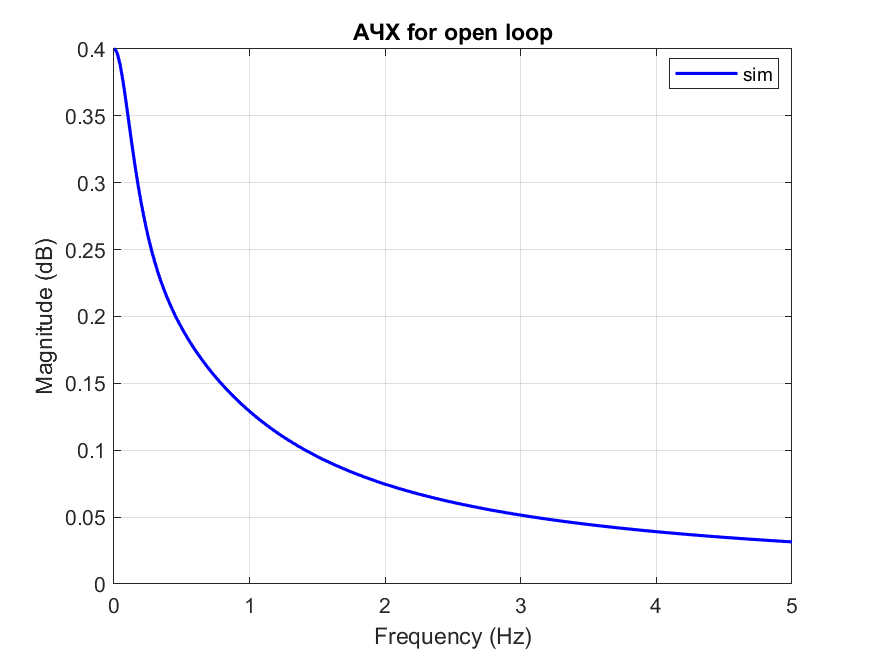
\includegraphics[width=0.7\textwidth]{freq_ampl2_closed1.png}
    \caption{АЧХ для разомкнутой системы, $k=1$}
\end{figure}
\begin{figure}[ht]
    \centering
    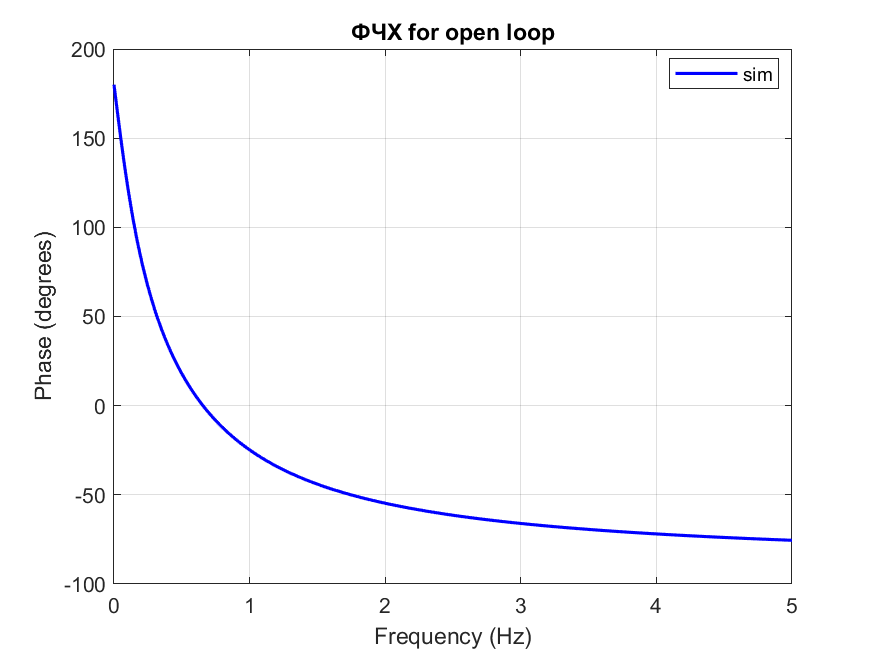
\includegraphics[width=0.7\textwidth]{freq_phase2_closed1.png}
    \caption{ФЧХ для разомкнутой системы, $k=1$}
\end{figure}

График ФЧХ начинается со сдвига в $180^\circ$, и как этой частоте $\omega_{crit}$ у нас будет располагаться ближайшая точка от годографа к критической. А значит амплитуда для этой частоты:
$$
\frac{1}{A_3} = A(\omega_{crit}) = 0.4
$$
$$
A_3 = \frac{1}{0.4} = 2.5
$$
Значит, получается, что запас амплитуды равен критическому значению коэффициента $k_{crit}$.

\newpage
\subsection{Переходные функции}
\begin{figure}[ht]
    \centering
    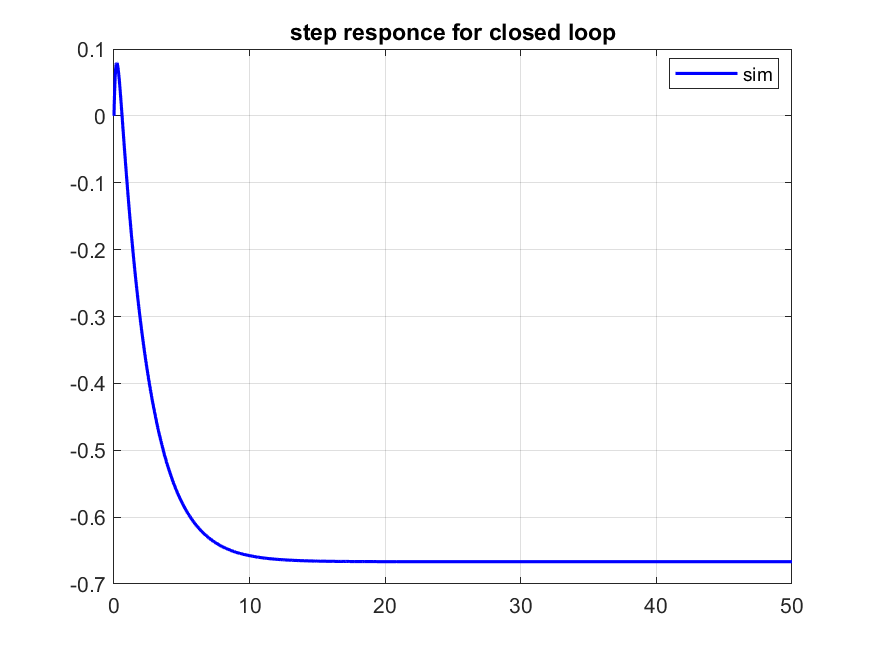
\includegraphics[width=0.7\textwidth]{step_responce21_closed1.png}
    \caption{Переходная функция для замкнутой системы, $k=1$}
\end{figure}
\begin{figure}[ht]
    \centering
    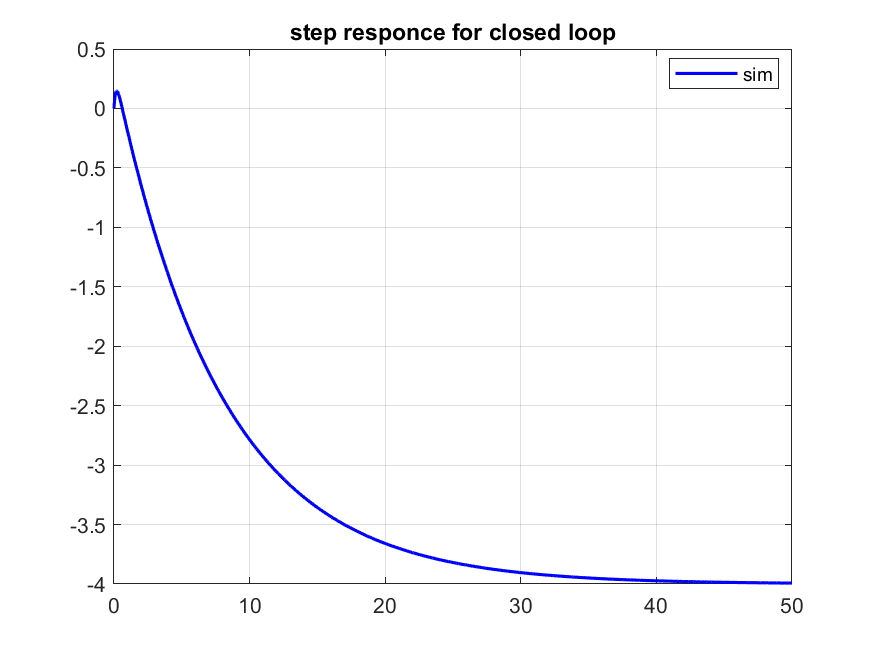
\includegraphics[width=0.7\textwidth]{step_responce22_closed1.png}
    \caption{Переходная функция для замкнутой системы, $k=2$}
\end{figure}
\begin{figure}[ht]
    \centering
    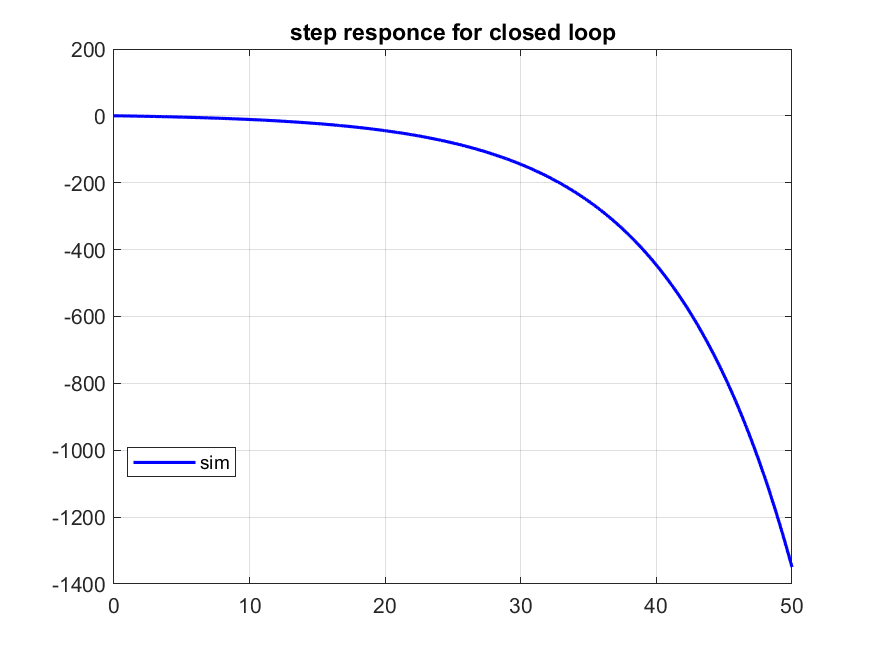
\includegraphics[width=0.7\textwidth]{step_responce23_closed1.png}
    \caption{Переходная функция для замкнутой системы, $k=3$}
\end{figure}
\begin{figure}[ht]
    \centering
    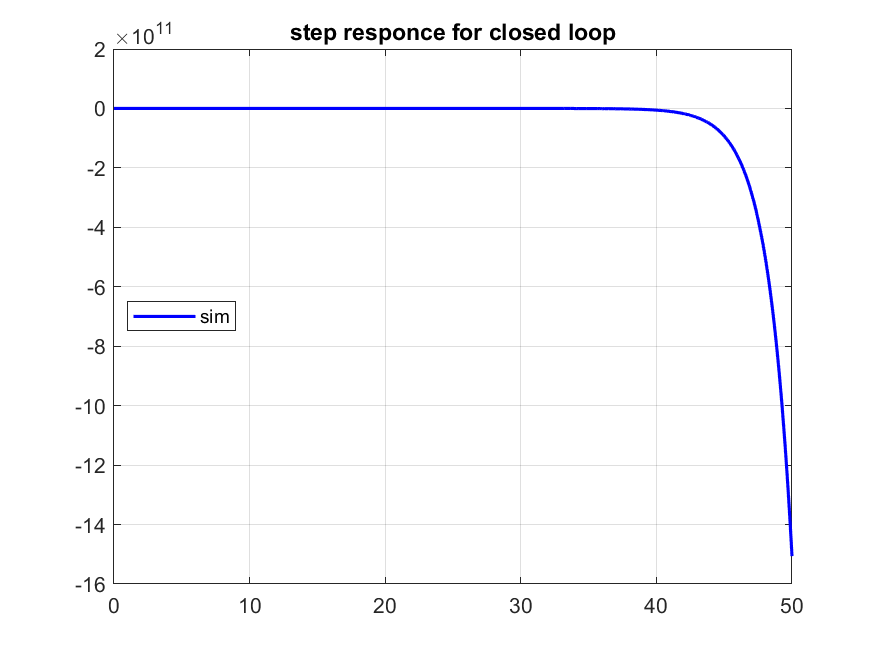
\includegraphics[width=0.7\textwidth]{step_responce24_closed1.png}
    \caption{Переходная функция для замкнутой системы, $k=6$}
\end{figure}

Можно заметить, что при значениях $k < 2.5$ - замкнутая система действительно устойчива, а при $k > 2.5$ - неустойчивая уже.
Разомкнутая система при любом $k$ будет оставаться устойчивой, потому что не имеет ни одного правого корня.

\newpage
\section{Передаточная функция $W_2$}
Для $k=1$:
$$
W_2(s) = \frac{-9s^3+16s^2-6s}{10s^3+12s^2+5s+1}
$$
Рассчитаем полюса: $\lambda_{1,2,3} \approx \{-0.68, -0.26\pm 0.28j \}$, значит разомкнутая система будет устойчива. 

\newpage
Построим для неё годографы, с разными $k$:
\begin{figure}[ht]
    \centering
    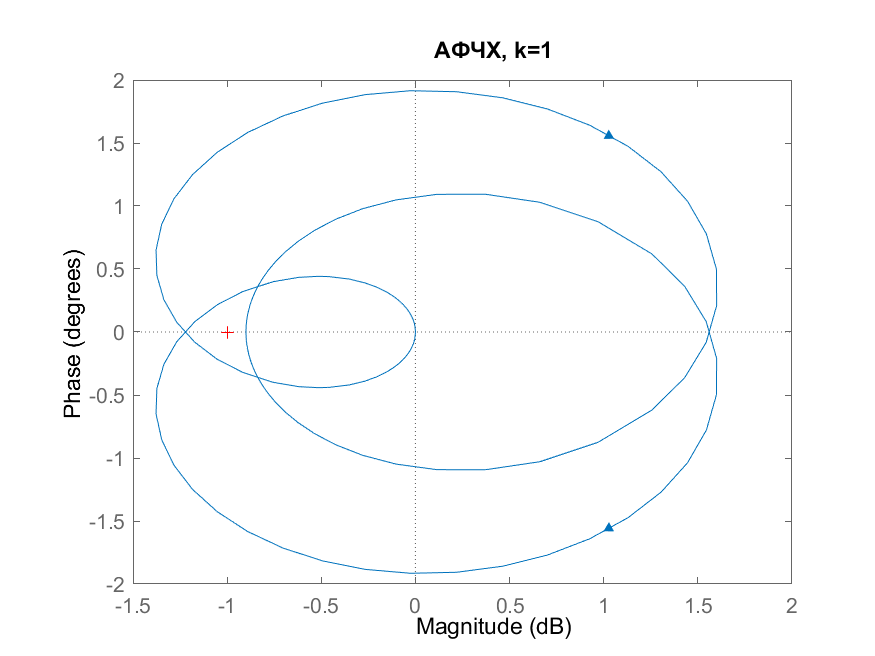
\includegraphics[width=0.7\textwidth]{nyquist_task21_object2.png}
    \caption{Годограф Найквиста для разомкнутой системы, $k=1$}
\end{figure}
\begin{figure}[ht]
    \centering
    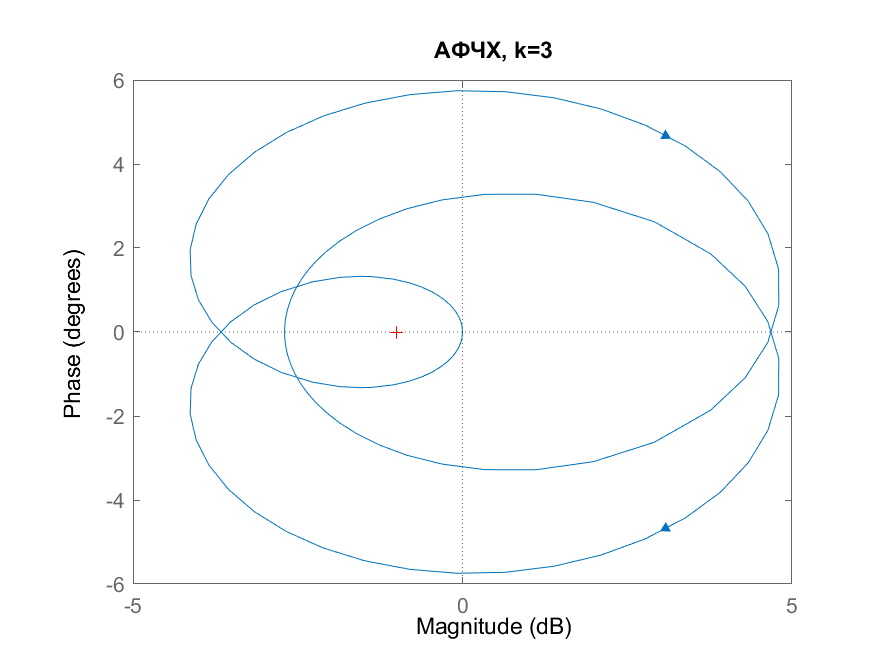
\includegraphics[width=0.7\textwidth]{nyquist_task22_object2.png}
    \caption{Годограф Найквиста для разомкнутой системы, $k=3$}
\end{figure}
\newpage
\begin{figure}[ht]
    \centering
    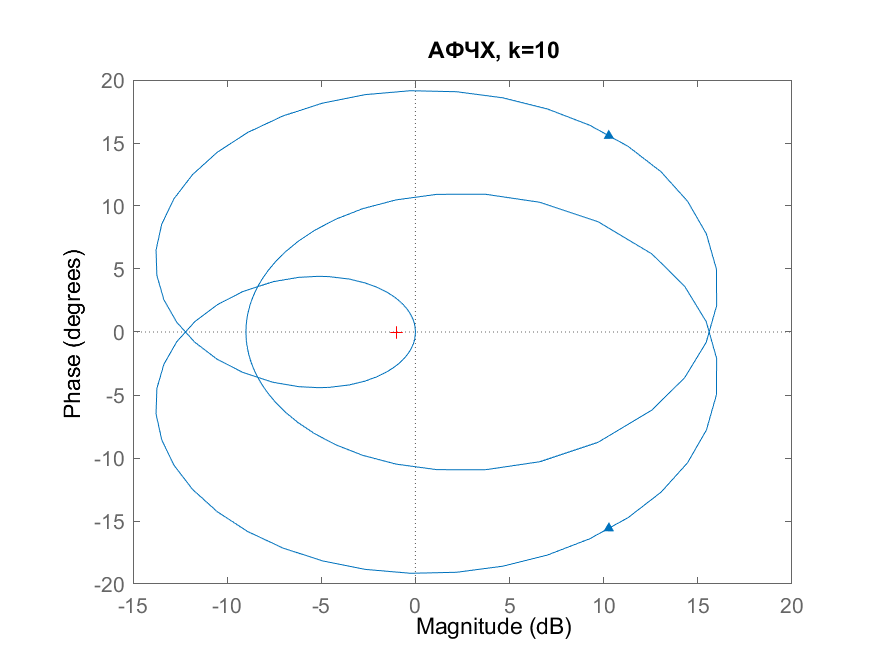
\includegraphics[width=0.7\textwidth]{nyquist_task23_object2.png}
    \caption{Годограф Найквиста для разомкнутой системы, $k=10$}
\end{figure}
\begin{figure}[ht]
    \centering
    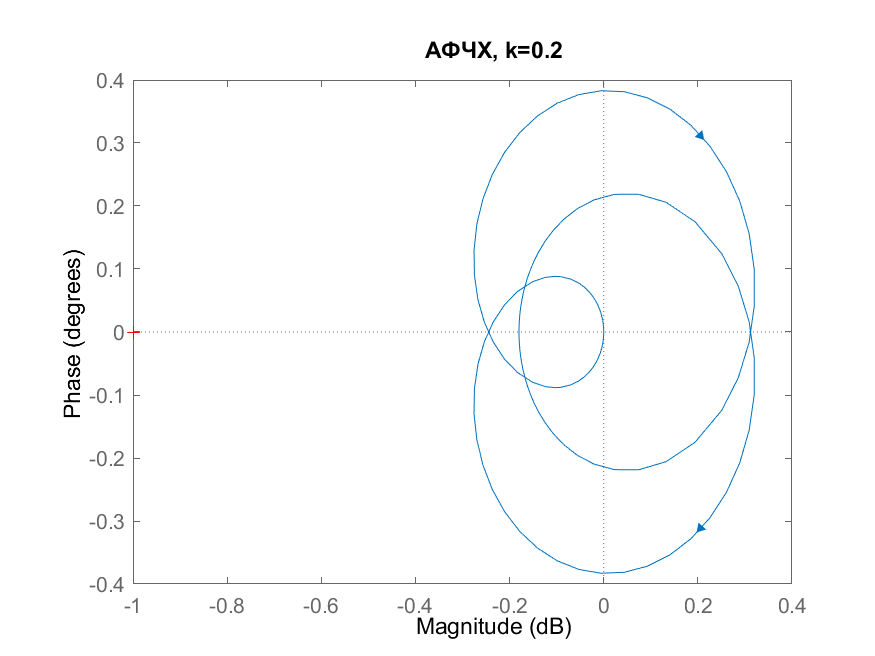
\includegraphics[width=0.7\textwidth]{nyquist_task26_object2.png}
    \caption{Годограф Найквиста для разомкнутой системы, $k=0.2$}
\end{figure}
\newpage
\begin{figure}[ht]
    \centering
    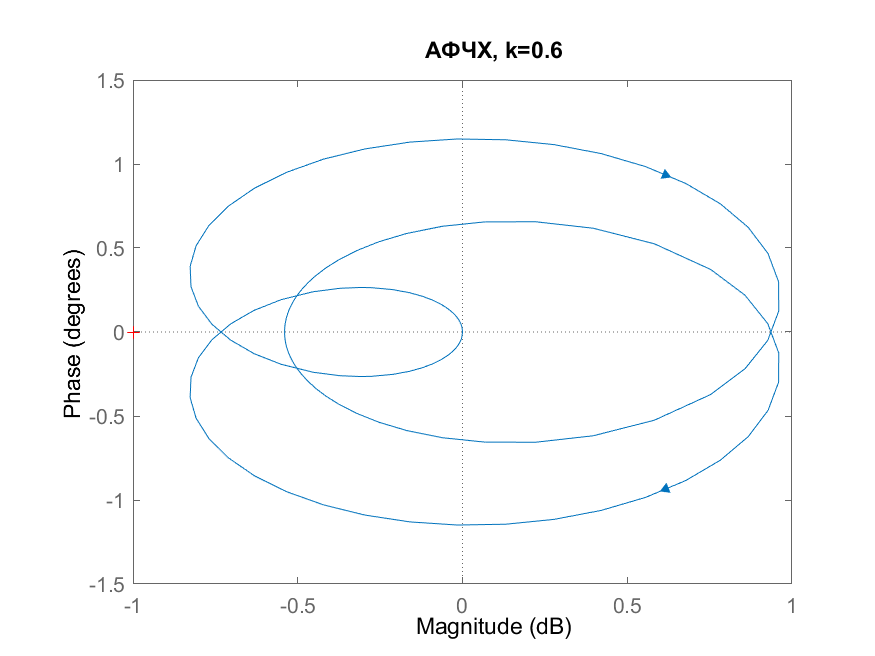
\includegraphics[width=0.7\textwidth]{nyquist_task24_object2.png}
    \caption{Годограф Найквиста для разомкнутой системы, $k=0.6$}
\end{figure}
\begin{figure}[ht]
    \centering
    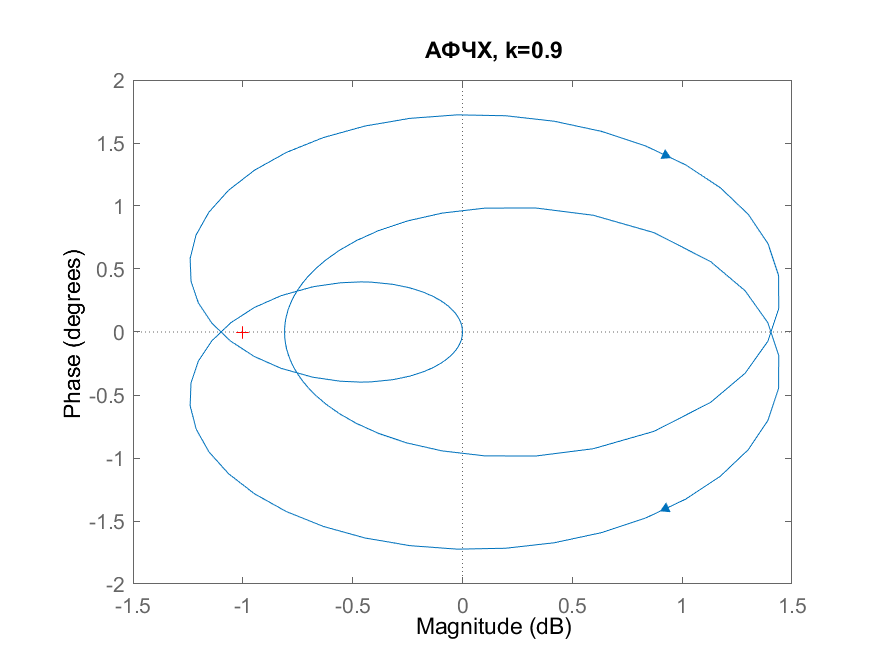
\includegraphics[width=0.7\textwidth]{nyquist_task27_object2.png}
    \caption{Годограф Найквиста для разомкнутой системы, $k=0.9$}
\end{figure}

Выходит, что коэффициент $k$ влияет на кривую годографа, расширяя её вдоль мнимой и вещественной оси. Уже при при $0.9 < k < 1$ мы начинаем получать 4 оборота по часовой стрелке, а значит +4 неустойчивых полюса для замкнутой системы, это  диапазон $k$  мы далее уточним при аналитике.
При бОльших $k > 1$ мы получаем +3 дополнительных нейстойчивых полюса для замкнутой системы, а при $k < 0.9$  - наша критическая точка и вовсе покидает годограф, он прилично сжимается. 

В итоге мы получили три диапазона для $k$, которые надо уточнить и проверить.
Чтобы узнать $k_{crit}$, посмотрим на критерий Гурвица:

$$
    W_{1,closed} = \frac{W_1}{1+W_1} = \frac{k(-9s^3 + 16s^2 -6s)}{(10-9k)s^3 + (12+16k)s^2 + (5-6k)s + 1 }
$$
Получим следующую систему:
$$
    \begin{cases}
        10-9k > 0 \\
        12+16k > 0 \\
        5-6k > 0 \\
        (12+16k)(5-6k) > (10-9k)
    \end{cases} \to
    -0.64 < k < 0.815
$$
Но отрицательные значения мы не рассматриваем, поэтому по критерию Гурвица система будет асимптотически устойчива при $0 < k < 0.815$,
так как до этого значения годограф не захватывает точку $(-1, 0)$, а значит не добавляет дополнительные неустойчивые полюса.
\newpage
\subsection{Частотные характеристики}
Построим ФЧХ,АЧХ для нашей системы при $k=1$, не имеет смысла строить для других $k$, ибо они лишь будут масштабировать АЧХ, фазовые сдвиги при этом будут оставаться теми же.
\begin{figure}[ht]
    \centering
    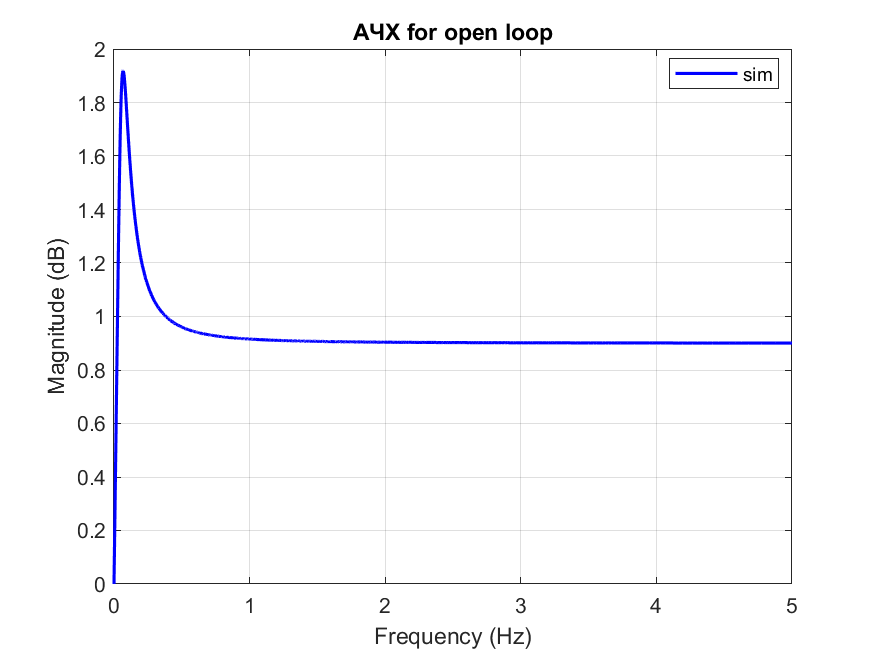
\includegraphics[width=0.7\textwidth]{freq_ampl2_closed2.png}
    \caption{АЧХ для разомкнутой системы, $k=1$}
\end{figure}
\begin{figure}[ht]
    \centering
    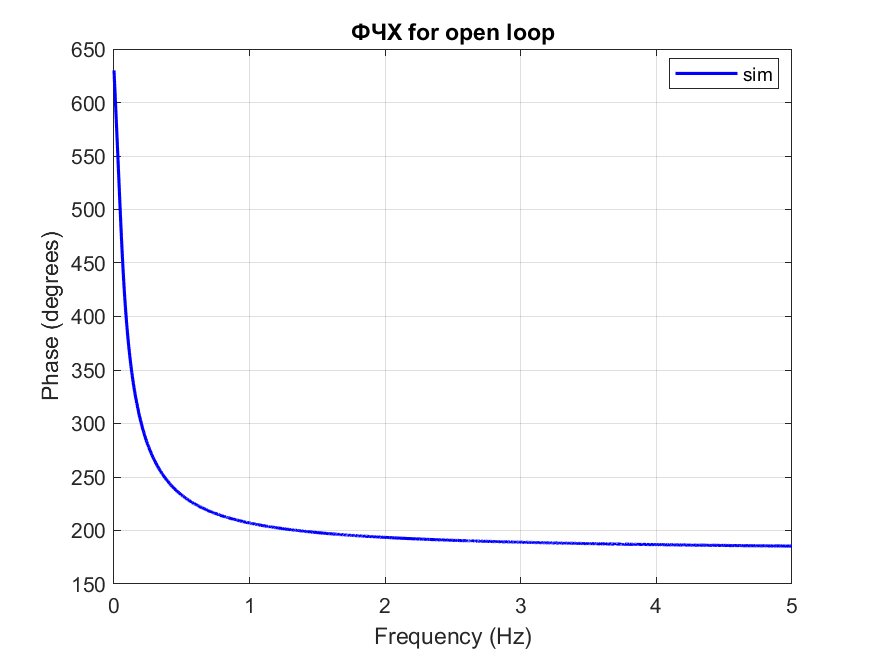
\includegraphics[width=0.7\textwidth]{freq_phase2_closed2.png}
    \caption{ФЧХ для разомкнутой системы, $k=1$}
\end{figure}

График ФЧХ начинается со сдвига в $630^\circ$ и снижается до $180^\circ$ асимптотическим образом. Значит в $180^\circ$ мы никогда не попадём, поэтому
ищем другой критический отрезок, у нас здесь остаётся только $540^\circ$. 

Однако стоит заранее остановить наш порыв найти запас по амплитуде, поскольку его нельзя определить для системы, которая уже при $k=1$ в замкнутом виде неустойчива. 
Поэтому с помощью частотных характеристик нам нельзя определить диапазон коэффицциента П-регулятора $k$. 

Тогда с помощью $\textrm{allmargin}$ получим список критических коэффициентов П-регулятора:
$$
    k_{max1} \approx 0.8156, \tab k_{max2} \approx 1.1111
$$

Мы уже нашли через критерий Гурвицца $k_{max1}$, а вместе со вторым коэффииентом мы теперь можем обозначить диапазоны для $k$:
\begin{enumerate}
    \item $k\in(0.00 ; 0.815)$ - замкнутая система будет иметь 0 неустойчивых полюсов.
    \item $k\in(0.815 ; 1.1111)$ - замкнутая система будет иметь 4 неустойчивый полюса (изначально система была устойчива). 
    \item $k\in(1.1111 ; +\infty)$ - замкнутая система будет иметь 3 неустойчивый полюса (изначально система была устойчива). 
\end{enumerate}

% В нём $\omega_{crit} \approx 0.031879$, тогда $A(\omega_{crit}) \approx 1.22901$
% $$
% A_3 = \frac{1}{A(\omega_{crit})} \approx 0.814
% $$
% Значит, получается, что запас амплитуды примерно равен критическому значению коэффициента $k_{crit}$. Я уверен, что они должны равняться, но просто нужно шаг уменьшить, нам и такой точности будет достаточно.



\newpage
\subsection{Переходные функции}
\begin{figure}[ht]
    \centering
    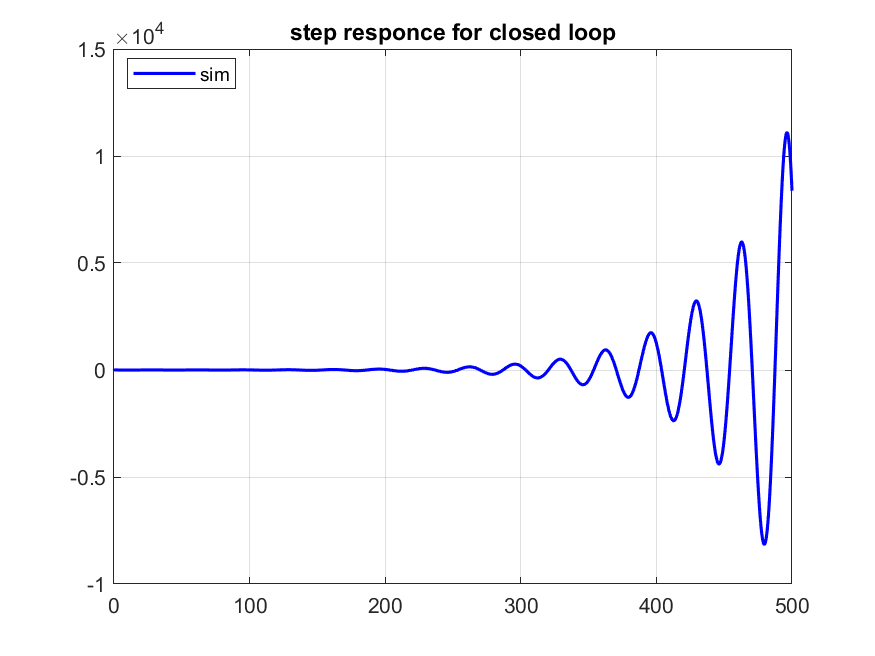
\includegraphics[width=0.7\textwidth]{step_responce21_closed2.png}
    \caption{Переходная функция для замкнутой системы, $k=1$}
\end{figure}
\begin{figure}[ht]
    \centering
    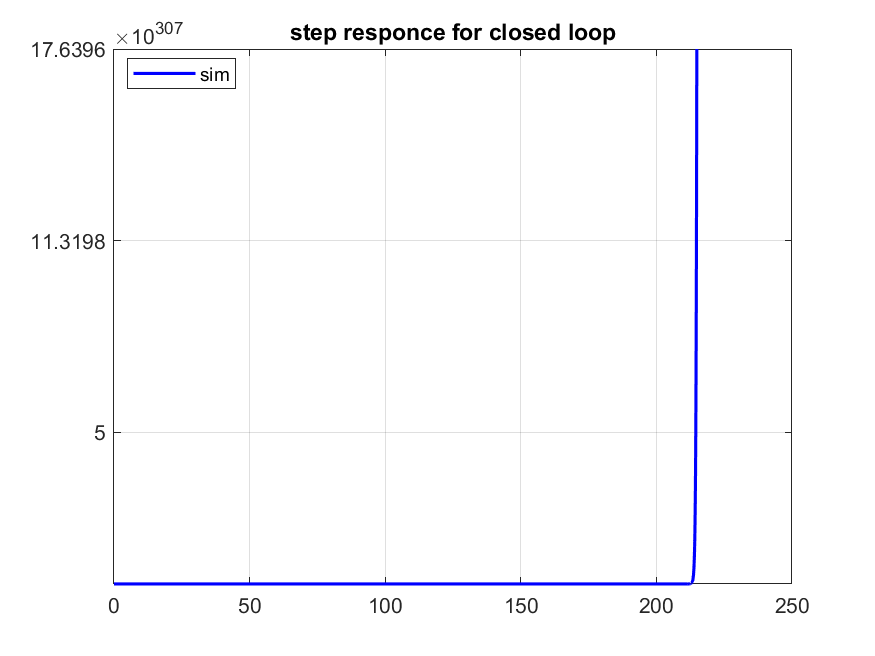
\includegraphics[width=0.7\textwidth]{step_responce22_closed2.png}
    \caption{Переходная функция для замкнутой системы, $k=3$}
\end{figure}

\newpage
\begin{figure}[ht]
    \centering
    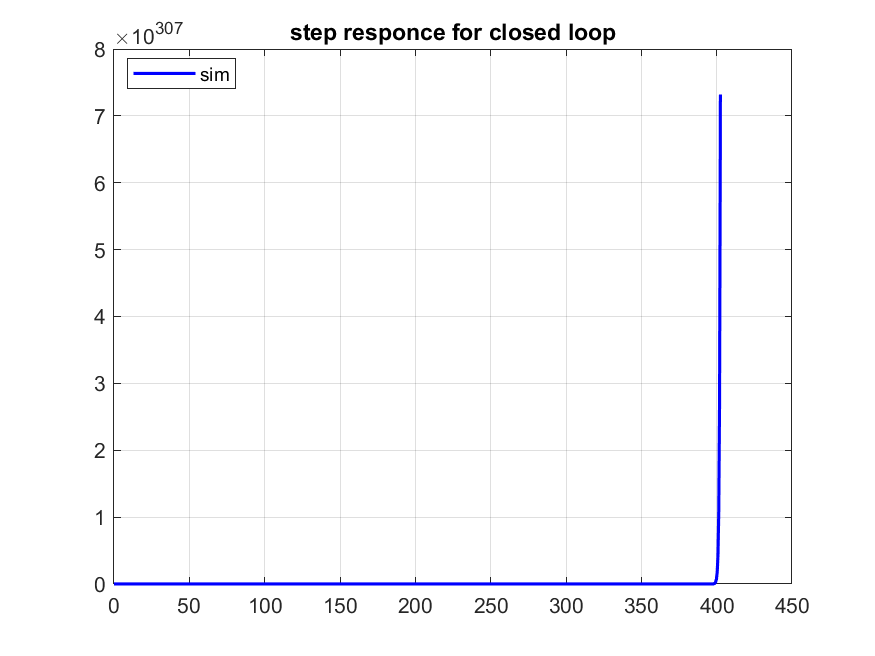
\includegraphics[width=0.7\textwidth]{step_responce23_closed2.png}
    \caption{Переходная функция для замкнутой системы, $k=10$}
\end{figure}
\begin{figure}[ht]
    \centering
    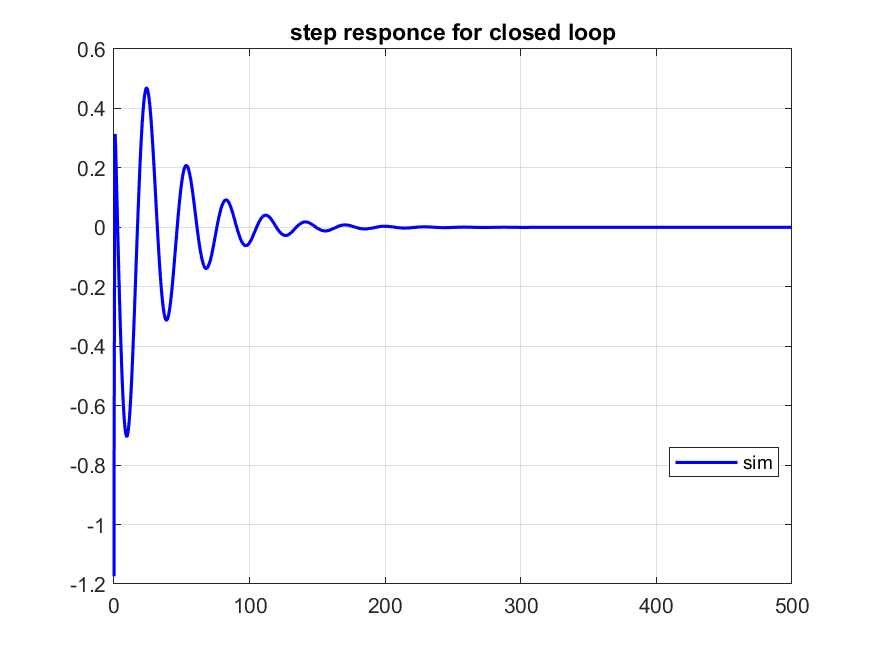
\includegraphics[width=0.7\textwidth]{step_responce24_closed2.png}
    \caption{Переходная функция для замкнутой системы, $k=0.6$}
\end{figure}
\newpage
\begin{figure}[ht]
    \centering
    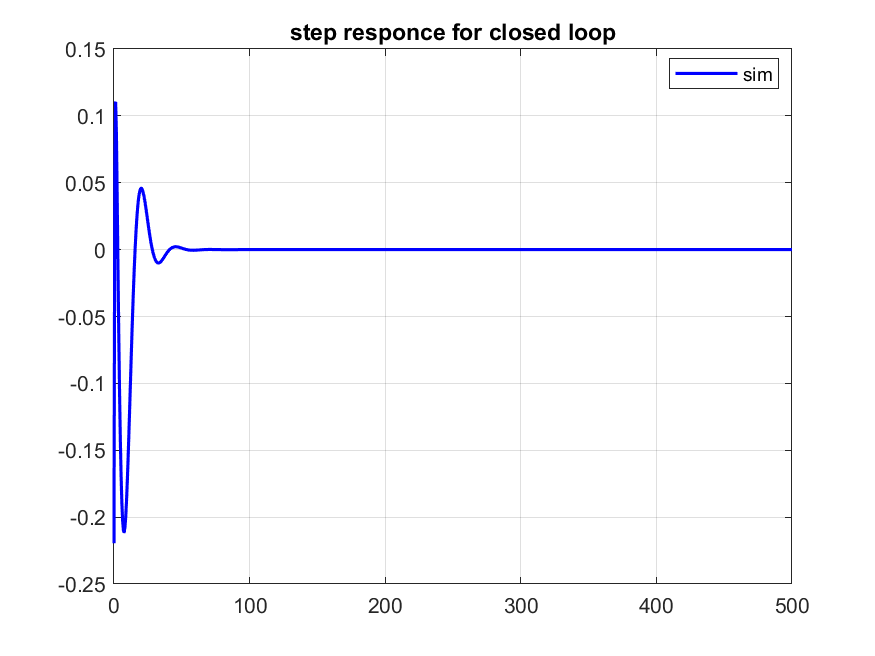
\includegraphics[width=0.7\textwidth]{step_responce26_closed2.png}
    \caption{Переходная функция для замкнутой системы, $k=0.2$}
\end{figure}
\begin{figure}[ht]
    \centering
    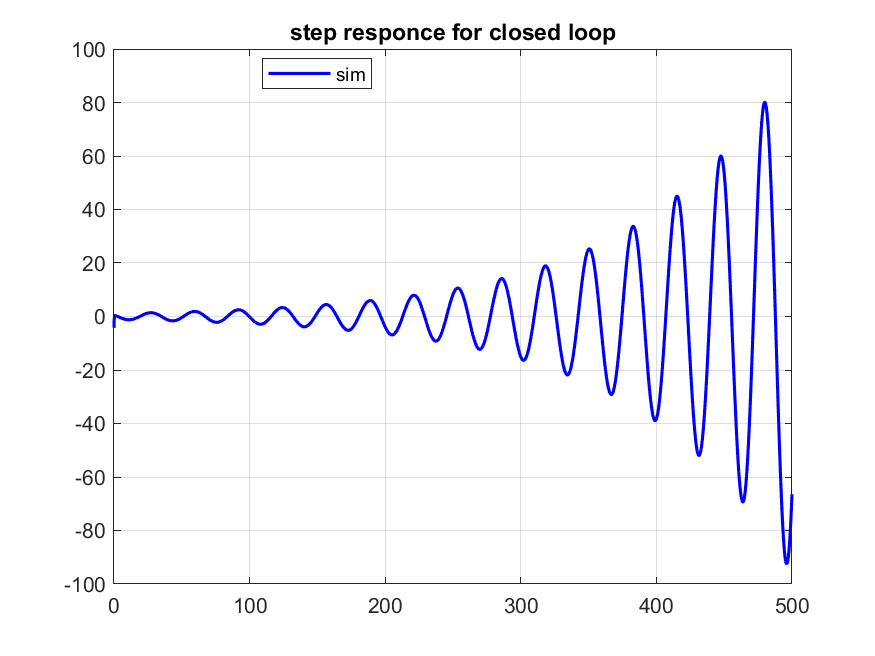
\includegraphics[width=0.7\textwidth]{step_responce27_closed2.png}
    \caption{Переходная функция для замкнутой системы, $k=0.9$}
\end{figure}

Можно заметить, что при значениях $0 < k < 0.815$ - замкнутая система действительно устойчива, а при $k > 0.815$ - неустойчивая уже, причём с разным количество неустойчивых полюсов.
Разомкнутая система при любом $k$ будет оставаться устойчивой, потому что не имеет ни одного правого корня.



\endinput